%%%%%%%%%%%%%%%%%%%%%%%%%%%%%%%		CHAP 4		%%%%%%%%%%%%%%%%%%%%%%%%%%%%%%%

\chapter{Data Analysis procedures}
\label{cha:4}
 Early stage data have also been analysed.
 In particular, event reconstruction techniques were developed and tested from scratch: %
 they are implemented in a purpose-built data analysis software, which studies signals acquired %
 from the water PMTs.
 The code's algorithm relies on individual pulse analysis and it is largely focuses on the rejection of %
 background with respect to event signals.
 These data analysis procedures are illustrated in this chapter, while meaningful results %
 are presented in the following chapter.
 Some of the methods could be employed into a more complete analysis %
 framework, valid even for the future phases of the experiment.

%\section{Data structure}

 The Main DAQ (see section~ref) is programmed to create a new \emph{Run} every time the Chain is %
 stopped and restarted.
 Due to being an R\&D phase, the DAQ has been improved in various occasion during data taking, %
 hence the size and the number of post-processed files, that constitute the \emph{Runs}, are not constant.
 Each file is a ROOT file containing the PMT data collected, in the way explained in section~ref.
 The buffer retrieved from the VME bards is properly split for each trigger signal, in that each %
 set of data consists of 80~$\mu$s worth of digitised signal.
 A file holds 383 full buffers and this translates to 1532 triggers: the effective time carried by %
 a single file is \np{122.560}~ms.

\section{Individual pulse analysis}

 The data analysis software scans all the post-processed time profile which the \emph{Run} consists of, %
 as the one shown in Fig.~\ref{fig:profile}, sorted by trigger and PMT number.
 Any peak above a certain voltage threshold, $V_T$, is selected and an enclosing time window %
 of a predefined length, $L$, is trimmed around it.
 A length of $L = 100$~samples was chosen, resulting in a \np{0.8}~$\mu$s long window.
 The position of the peak inside this window was set to 20\% of its length, i.e. the peak is always %
 set at \np{0.16}~$\mu$s from the beginning of the time window.
 These subsets of data are being called \emph{pulses} and are collected in another ROOT file.
 The choice of window length and the peak position is the result of a compromise between speed of the code, %
 memory usage and loss of physical information.
 In fact, many pulses shows consecutive multiple peaks, as the one in Fig.~\ref{fig:pulse}, mainly given by %
 light reflections in the water tank.

 Each pulse is individually analysed and processed by a routine of algorithms.
 As a result, a set of values, typical of the pulse\footnote{I don't like this.}, are gathered from every pulse, %
 in addition to Veto and MRD coincidences.
 These quantities, outlined in Fig.~\ref{fig:pulseana}, are useful for following analysis and they are:

%\begin{center}
%\begin{varwidth}{\textwidth}
\begin{description}
%  \item[Length] of the pulse array;
%  \item[Trigger] number and PMT ID;
  \item[\bfseries Baseline] is given by the average of first 10 points of the pulse; %
    this value is then subtracted from the whole array.
  \item[\bfseries Height] is the height of the peak (maximum) with respect to the zero.
  \item[\bfseries Peak to valley] it is the time distance from the peak to the valley (minimum);
  \item[\bfseries Start] is position of the 25\% of the rising edge of the pulse, estimated with %
    precision using cubic interpolation\footnotetext{The algorithm looks for four points around the %
    threshold which are used to define a cubic function. Using Newton's method, the time position %
    is found.}.
  \item[\bfseries Width] is the time that spans from Time to the 5\% of the falling edge %
    of the pulse, calculated using the same algorithm employed for Time.
  \item[\bfseries Charge] is the sum of the 5 points around peak, weighted by the bin width.
  \item[\bfseries Energy] is the sum of the points form Time to Time+Width, with bin weight.
  \item[\bfseries Area] is the area of the modulus of the pulse.
  \item[\bfseries Time of flight] is the time difference between Time and RWM signal.
  \item[\bfseries Previous] is the Time of the previous pulse, if from the same PMT.
    \color{red}
\end{description}
%\end{varwidth}
%\end{center}


 \begin{figure}
   \centering
   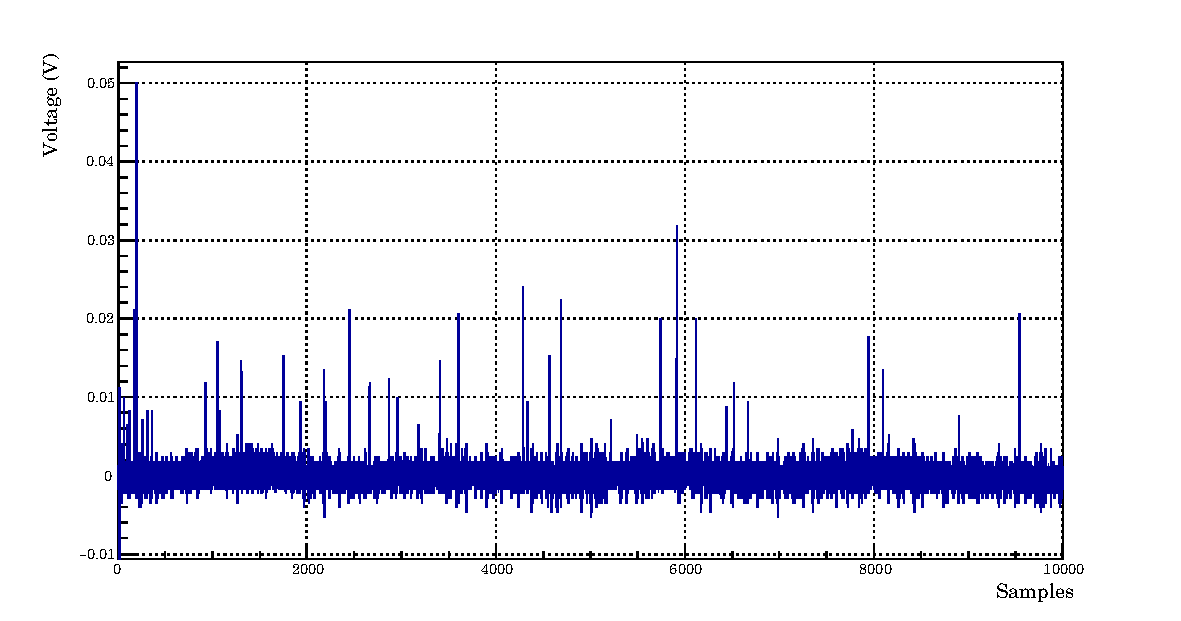
\includegraphics[scale=0.7]{pics/timeprofile.pdf}
   \caption{Time profile of a single trigger: the signals of the sixty PMTs are here overlaid.}
   \label{fig:profile}
 \end{figure}

 \begin{figure}
   \centering
   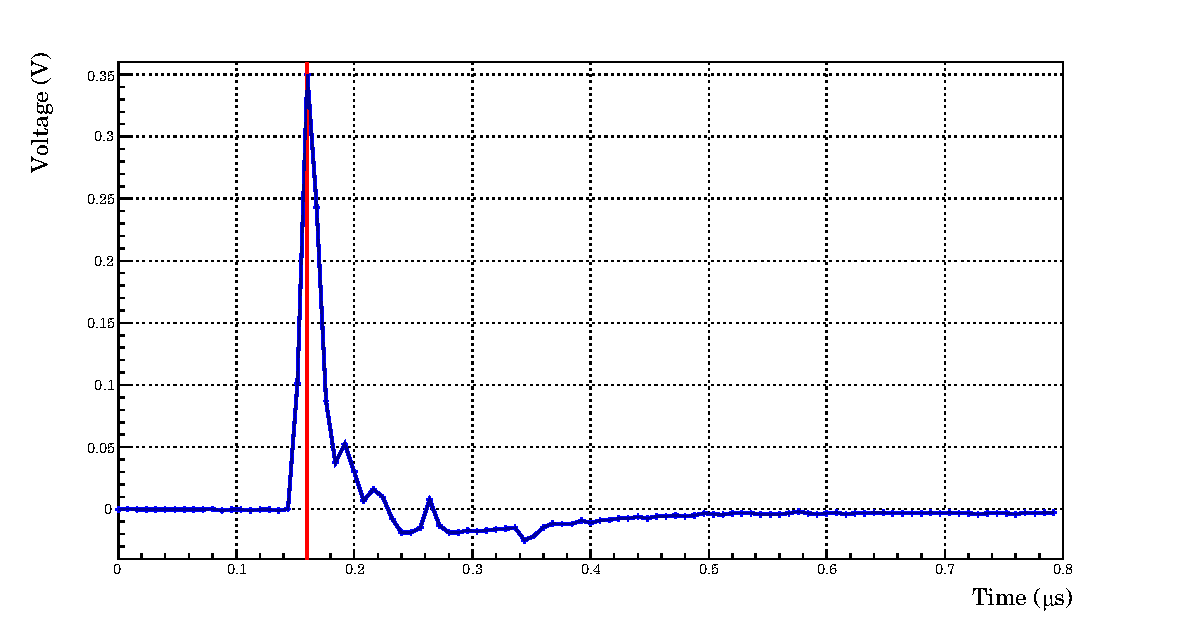
\includegraphics[scale=0.7]{pics/pulse.pdf}
   \caption{Time profile of a single pulse. The red line marks the 20\,\% of the window's length, at $\np{0.16}~\mu$s. %
     The first peak and the second peak are about forty nanoseconds apart, which is the time needed for the light to %
   travel back and forth inside the tank (see section~ref).}
   \label{fig:pulse}
 \end{figure}

\begin{figure}
  \centering
  \def\svgwidth{0.47\textwidth}
  \subfloat[From left to right: in green the \emph{BaseLine}, in orange the \emph{Peak Height}, %
  in purple the \emph{Width}, and in light blue the \emph{Peak to Valley} time distance.]%
  {\import{pics/}{timepoints.pdf_tex}} \qquad
  \def\svgwidth{0.47\textwidth}
  \subfloat[From left to right: in pink the \emph{Charge}, in blue the \emph{Energy}, and in gold the \emph{Area}.%
  These three integrals cross over each other in the purple region.]%
  {\import{pics/}{areapoints.pdf_tex}}
  \caption{Illustration of the pulse analysis values. The \emph{25\,\%} and \emph{5\,\% peak height} marks, %
  which define the \emph{Start} and \emph{End} of the signal, are common to both diagrams. The dashed lines represent %
  the cubic interpolations.}
  \label{fig:pulseana}
\end{figure}

\section{Event definition}

 For every Trigger, the time distribution of the peaks is also studied, as well as the time coincidences %
 between the PMTs signals: a time allowance of $\np{0,8}~\mu$s is considered to count of pulses happening %
 simultaneously; this easily translates to the number of PMTs fired at the same time.
 When the latter exceeds a defined threshold, $N_{PMT}$, then an \emph{Event} is appointed and its precise time %
 position is afterwards estimated by a weighted average of the adjacent coincidences.
 The multiplicity of an Event is a good indicator of the nature of the detected interaction.
 As discussed in section~ref, a cosmic muon, likely coming from above, would project the Cherenkov radiation on the %
 bottom of the tank, thus lighting the majority of the water PMTs.
 On the other hand, a muon arisen from the interaction of a beam neutrino with a nucleon would emit gammas %
 along the beam direction: only a portion of the light cone could be captured.
 Even natural radioactivity, from radionuclide in the glass of the phototubes, can trigger some detectors, although %
 this event are readily filtered by a proper value of $N_{PMT}$.
 An high-multiplicity event is exemplified in Fig.~\ref{fig:event}.

  \begin{figure}
   \centering
   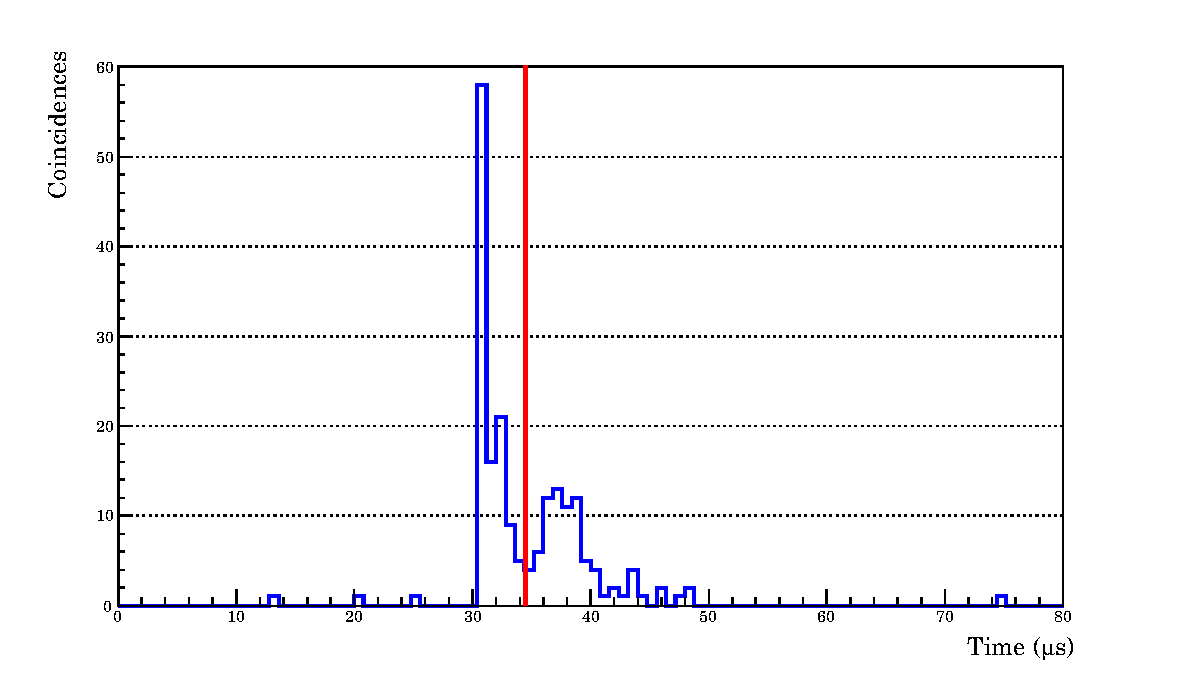
\includegraphics[scale=0.7]{pics/coincidences.pdf}
   \caption{This histogram is filled with the Start time of each pulse belonging to the same trigger.
     An high multiplicity is found near $\np{31}~\mu$s. In this particular case, the time distribution of %
     the signals is quite long: the light in the tank lasts for about twenty microseconds.
     The red line marks the weighted average of the coincidences, which is $\np{34.51}~\mu$s in this example.}
   \label{fig:event}
 \end{figure}

\section{Signal and noise discrimination}

\textcolor{red}{Bad english here.}
 Not all the pulses found in a trigger belong to the Event.
 For instance, in Fig.~\ref{fig:event} there are four pulses far from the main pulse cluster.
 These might be likely generated by noise sources and therefore they are meaningless.
 In order to discriminate the pulses, time window is defined around the Event time position.
 Every pulse that falls within this interval is designated as a \emph{signal}; otherwise it is \emph{noise}.

 \textcolor{blue}{I need a picture of the rejection time window and a picture of $N_{PMT}$ freq.}

 Discriminating signal from background is a step of utmost importance for data analysis.
 In order to find the best value of the parameter (see section~ref), these have been varied, thus the data %
 have been analysed various times.
 Twelve combination were chosen and they are listed in Tab.~\ref{tab:thr_var}.

 \begin{wraptable}{r}{0.4\textwidth}
  \caption{The combination of the employed thresholds are here listed.}
  \label{tab:thr_var}
  \centering
  \footnotesize
  \begin{tabular}{ccc}
    \toprule
    \textbf{$V_T$}	& \textbf{$N_{PMT}$}	& \textbf{$\Delta_T$}	\\
    (V)	 		& 			& ($\mu$s)			\\
    \midrule
    \textbf{\np{0.02}}	& \textbf{10}		& \textbf{\np{4.0}}		\\
    \midrule
    \np{0.005}		& 10			& \np{4.0}			\\
    \np{0.01}		& 10			& \np{4.0}			\\
    \np{0.05}		& 10			& \np{4.0}			\\
    \np{0.10}		& 10			& \np{4.0}			\\
    \midrule
    \np{0.02}		& 15			& \np{4.0}			\\
    \np{0.02}		& 30			& \np{4.0}			\\
    \np{0.02}		& 50			& \np{4.0}			\\
    \midrule
    \np{0.02}		& 10			& \np{5.0}			\\
    \np{0.02}		& 10			& \np{3.0}			\\
    \np{0.02}		& 10			& \np{2.0}			\\
    \np{0.02}		& 10			& \np{1.0}			\\
    \bottomrule
  \end{tabular}
 \end{wraptable}

\section{Data selection}

 Being an R\&D stage, the data acquisition has not been methodic and continuous, but notwithstanding %
 high statistics were achieved most of the time.
 Three distinctive couples of consecutive runs were selected as model data set, with the intention to %
 outline the best data analysis procedures.
 These are
\begin{center}
\begin{varwidth}{\textwidth}
\begin{itemize}
%    \centering
    \small
  \item[\bfseries R93/R94] beam off, trigger random	
  \item[\bfseries R120/R121] after card synchronisation	
  \item[\bfseries R145/R146] PMT mounted on NCV		
\end{itemize}
\end{varwidth}
\end{center}
 and their characteristics are shown in Tab.~\ref{tab:runs}.

\begin{table}
  \caption{Runs selected for data analysis. They are composed of different numbers of file, resulting in %
    diverse number of triggers. Total time is the number of triggers times 80~$\mu$s.
    The listed memory sizes refer to the post-processed files.}
  \label{tab:runs}
  \footnotesize
  \centering
  \begin{tabular}{crcrr}
    \toprule
    \textbf{Run} & \textbf{N of files} & \textbf{N of Triggers} & \textbf{Total time} & \textbf{Data size} \\
    		 &      	&		& (ms)			& 	(MB)	            	\\
    \midrule	                                                                     
      93	 & 88	& \np{134816}	& \np{10785.280}	& $ \np{65027.961} $       	\\
      94	 & 54	& \np{82728}	& \np{6618.240}		& $ \np{41102.486} $       	\\
      120	 & 43	& \np{65876}	& \np{5270.080}		& $ \np{19887.893} $       	\\
      121	 & 15	& \np{22980}	& \np{1838.400}		& $ \np{6735.270}  $       	\\
      145	 & 80	& \np{122560}	& \np{9804.800}		& $ \np{37204.525} $       	\\
      146	 & 84	& \np{128688}	& \np{10295.040}	& $ \np{39050.909} $       	\\
    \bottomrule
  \end{tabular}
\end{table}
